\documentclass{article}
\usepackage[utf8]{inputenc}
\usepackage{graphicx}
\usepackage[main=greek,english]{babel}
\usepackage{adjustbox}
\newcommand\tab[1][1cm]{\hspace*{#1}}
\newcommand \en {\selectlanguage{english}}
\newcommand \gr {\selectlanguage{greek}}

\newcommand{\ApEn}{1.254729411772911}
\newcommand{\AVG}{0.8366083333333328}
\newcommand{\Bubble}{0.03238742763895071}
\newcommand{\RMSSD}{0.21656147967029465}
\newcommand{\Shannon}{4.732081187239775}
\newcommand{\SampEn}{2.0961923521046515}
\newcommand{\STD}{0.20614201146027678}
\newcommand{\meanApEn}{0.81}
\newcommand{\meanAVG}{0.71}
\newcommand{\meanRMSSD}{0.05}
\newcommand{\meanBubble}{0.01}
\newcommand{\meanShannon}{4.12}
\newcommand{\meanSampEn}{0.9}
\newcommand{\meanSTD}{0.88}
\newcommand{\Renyi}{6.661188009214217}
\newcommand{\meanRenyi}{6.17}

\begin{document}
\begin{figure}[h]
	\centering
	
\includegraphics[scale=.6]{homore.png}
\end{figure}
\noindent\hrulefill

\bigskip\bigskip\bigskip
\begin{center}
    \textbf{\Large \gr Ανάλυση Καρδιακού Ρυθμού }
\end{center}

\bigskip\bigskip
\bigskip

\noindent\hrulefill

\bigskip\bigskip
\textbf{\gr Βασικές Μετρήσεις:} \\
\par

\adjustbox{max width=\textwidth}{%
\begin{tabular}{c c c c} 

    \textbf{\gr Μέτρο}       &   \textbf{Μέτρηση}     &   \textbf{Μέση τιμή ασθενούς}      &   \textbf{Φυσιολογική τιμή}    \\
    \hline \\
    
 \en    AVG         &   \AVG         &   \meanAVG                 &   \en xxx                 \\
 \en    RMSSD       &   \RMSSD       &   \meanRMSSD               &   \en xxx                 \\
 \en    STD         &   \STD         &   \meanSTD                 &   \en xxx                 \\
\par
 \en    Shannon Entropy          &   \Shannon           &   \meanShannon              &   \en xxx                 \\
  \en   Renyi Entropy           &   \Renyi            &   \meanRenyi               &   \en xxx                 \\
 \en    Approximate Entropy     &   \ApEn       &   \meanApEn          &   \en xxx                 \\
 \en    Sample Entropy           &   \SampEn            &   \meanSampEn               &   \en xxx                 \\
 \en    Bubble Entropy           &   \Bubble            &   \meanBubble               &   \en xxx                 \\
 
\end{tabular}}

\newpage
\begin{center}
    \textbf{Περιοχές Σήματος προς Διερεύνηση:}
\end{center}

\bigskip\bigskip

\begin{figure}[h]
    \centering
	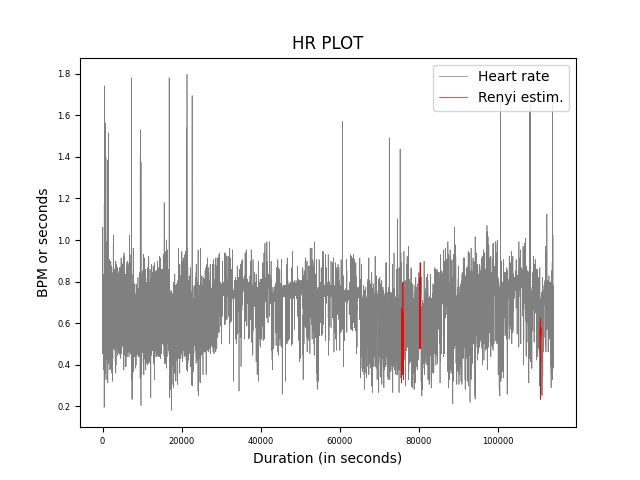
\includegraphics[scale=0.5]{document/congestive-heart-failure-rr-interval-database-1.0.0_223_240sec.jpeg}
 \caption{Καρδιογράφημα με εντοπισμό πιθανών επικίνδυνων περιοχών με βάση τη μετρική \en Renyi Entropy}
\end{figure}


\begin{figure}[h]
    \centering
	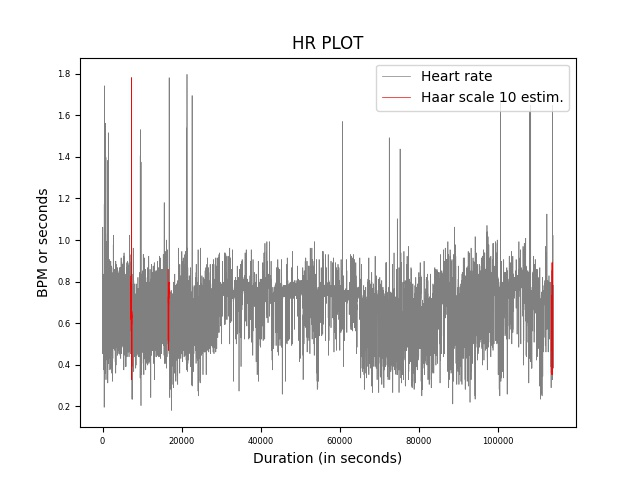
\includegraphics[scale=0.5]{document/Haar_scale_10_223_240sec.jpeg}
 \caption{Καρδιογράφημα με εντοπισμό πιθανών επικίνδυνων περιοχών με βάση τα κυματίδια \en Haar \gr σε κλίμακα εκτίμησης 10}
\end{figure}

\end{document}